There are three major systems for plotting in \R: \texttt{base}, \texttt{lattice}, and \texttt{gglot}. All three can do the same things, so you do not need to learn all of them. I will show you how to make graphs using \texttt{ggplot} which is very popular among \R users. In order to use it, we need to load the \texttt{ggplot2} library.

\subsection{Basic graphs}

We'll start out using the \texttt{base} functions to create plots. These might not be publication-ready but suffice for some basic exploration of the data.

\begin{lstlisting}
> x <- -10:10
> y <- x^2
> plot(y ~ x)

> # in a data frame
> data <- data.frame(x = x, y = y)
> with(data, plot(y ~ x))
\end{lstlisting}

\begin{figure}[h]
\centering
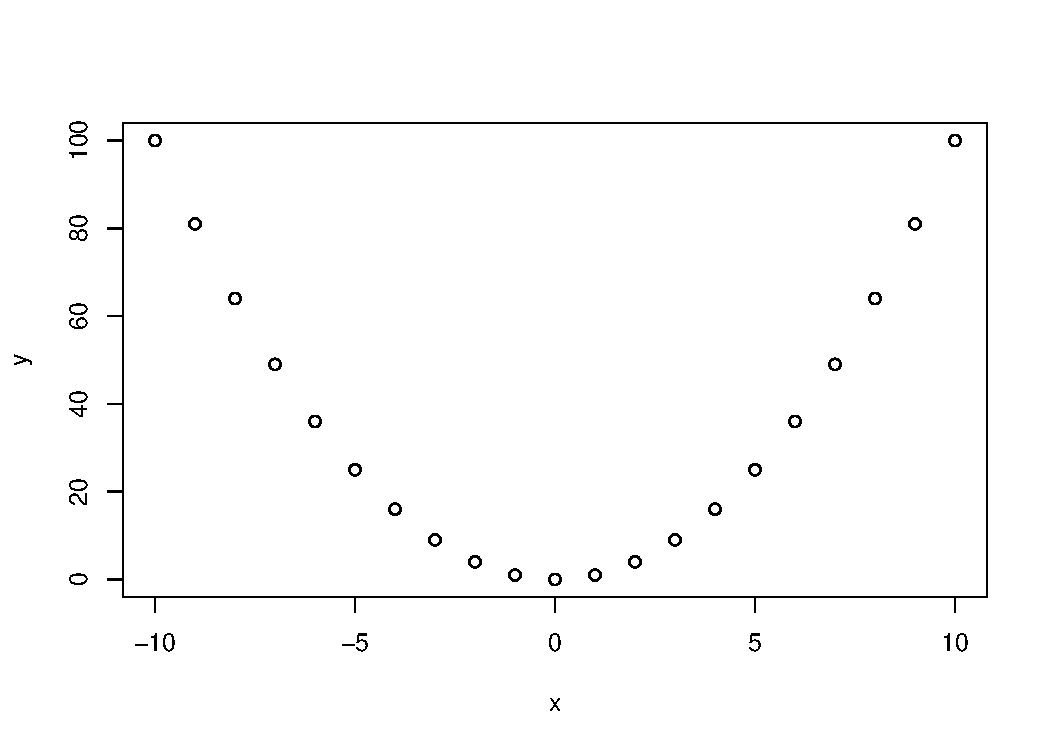
\includegraphics[width=4in]{plots/01.pdf} 
\end{figure}

To get a fast histogram we can do the following:

\begin{lstlisting}
> x <- rnorm(1000)
> hist(x, freq = FALSE)
\end{lstlisting}

\begin{figure}[h]
\centering
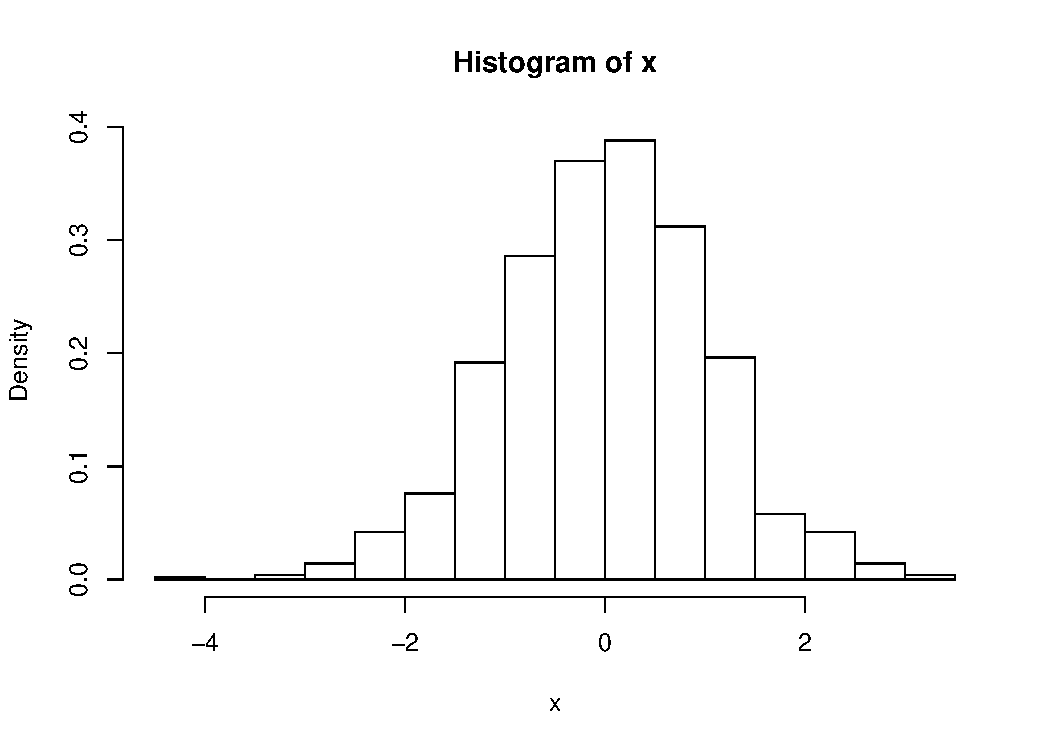
\includegraphics[width=4in]{plots/02.pdf} 
\end{figure}

\subsection{Scatterplots}

Let's start using \texttt{ggplot}. We're going to use a data set that is part of the \texttt{ggplot2} package. The data set \texttt{midwest} includes demographic information for counties in the Midwest.

\begin{lstlisting}
> library(ggplot2)
> data(midwest)

> colnames(midwest)
 [1] "PID"                  "county"               "state"               
 [4] "area"                 "poptotal"             "popdensity"          
 [7] "popwhite"             "popblack"             "popamerindian"       
[10] "popasian"             "popother"             "percwhite"           
[13] "percblack"            "percamerindan"        "percasian"           
[16] "percother"            "popadults"            "perchsd"             
[19] "percollege"           "percprof"             "poppovertyknown"     
[22] "percpovertyknown"     "percbelowpoverty"     "percchildbelowpovert"
[25] "percadultpoverty"     "percelderlypoverty"   "inmetro"             
[28] "category"   
\end{lstlisting}

\texttt{ggplot} relies on layers which are connected with the `+' sign. The first layer is created using the \texttt{ggplot} command on a data frame.

\begin{lstlisting}
> plot1 <- ggplot(midwest)
> plot1  # it's blank
\end{lstlisting}

To actually plot something we need to add another layer.

\begin{lstlisting}
# plot percentage of people with college degree vs percentage living below the poverty level
> plot1 <- ggplot(midwest) + 
+             geom_point(aes(x = percollege, y = percbelowpoverty))
> plot1
\end{lstlisting}

\begin{figure}[h]
\centering
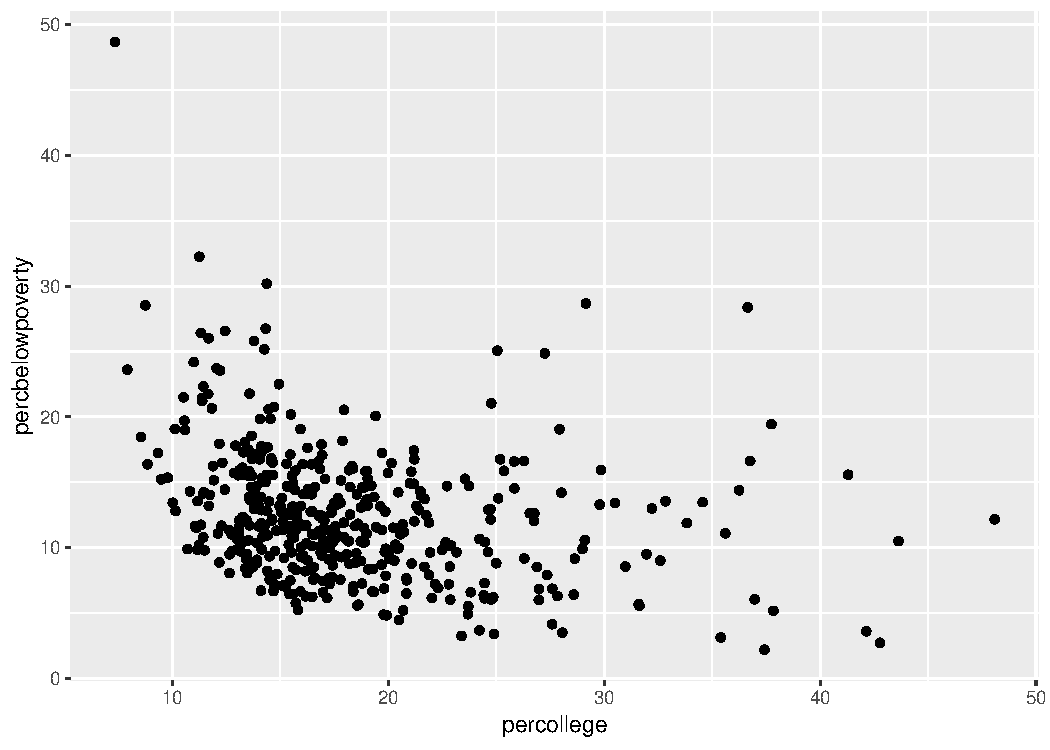
\includegraphics[width=4in]{plots/03.pdf} 
\end{figure}

Once a plot is created, it is pretty straight-forward to make changes to it. Let's say we want to add a title and change the axis labels.

\begin{lstlisting}
> plot1 <- plot1 +   # take plot1 and add
+            xlab("Percentage of people with college degree") +
+            ylab("Percentage of people below poverty line") +
+            ggtitle("College degrees and poverty")
> plot1
\end{lstlisting}

\begin{figure}[h]
\centering
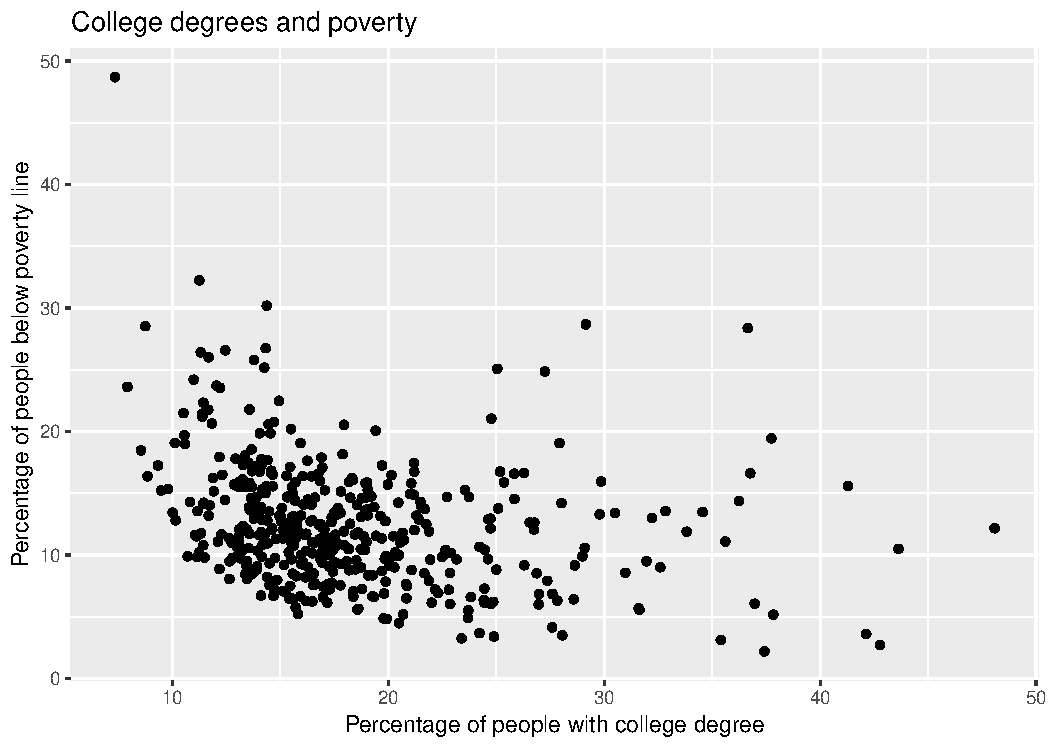
\includegraphics[width=4in]{plots/04.pdf} 
\end{figure}

We can add color by including a factor variable. In this case, let's color the observation by states.

\begin{lstlisting}
> midwest$state <- factor(midwest$state)  # needs to be a factor
> plot1 <- ggplot(midwest) +
+            geom_point(aes(x = percollege, y = percbelowpoverty, color = state)) +
+            xlab("Percentage of people with college degree") +
+            ylab("Percentage of people below poverty line") +
+            ggtitle("College degrees and poverty")
> plot1
\end{lstlisting}

\begin{figure}[h]
\centering
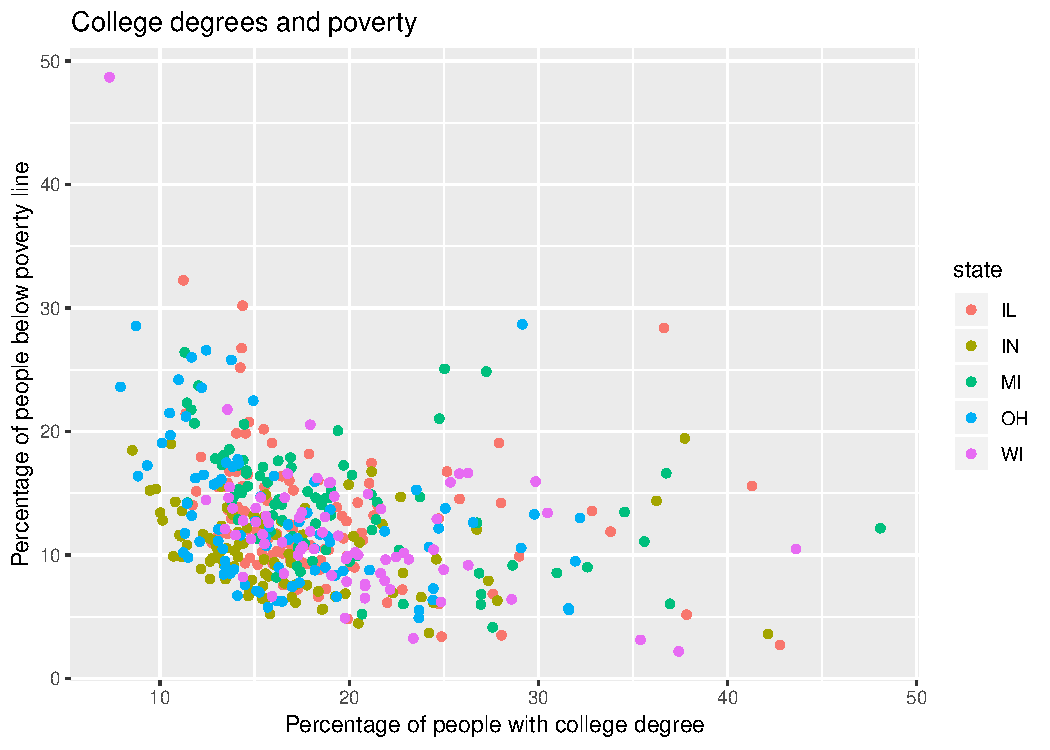
\includegraphics[width=4in]{plots/05.pdf} 
\end{figure}

Alternatively, we can also adjust the color, shape, and size of all points if we do so within \texttt{geom\_point} but outside \texttt{aes}.

\begin{lstlisting}
> plot1 <- ggplot(midwest) +
+            geom_point(aes(x = percollege, y = percbelowpoverty), col = "steelblue") +            
+            xlab("Percentage of people with college degree") +
+            ylab("Percentage of people below poverty line") +
+            ggtitle("College degrees and poverty")
> plot1
\end{lstlisting}

\begin{figure}[h]
\centering
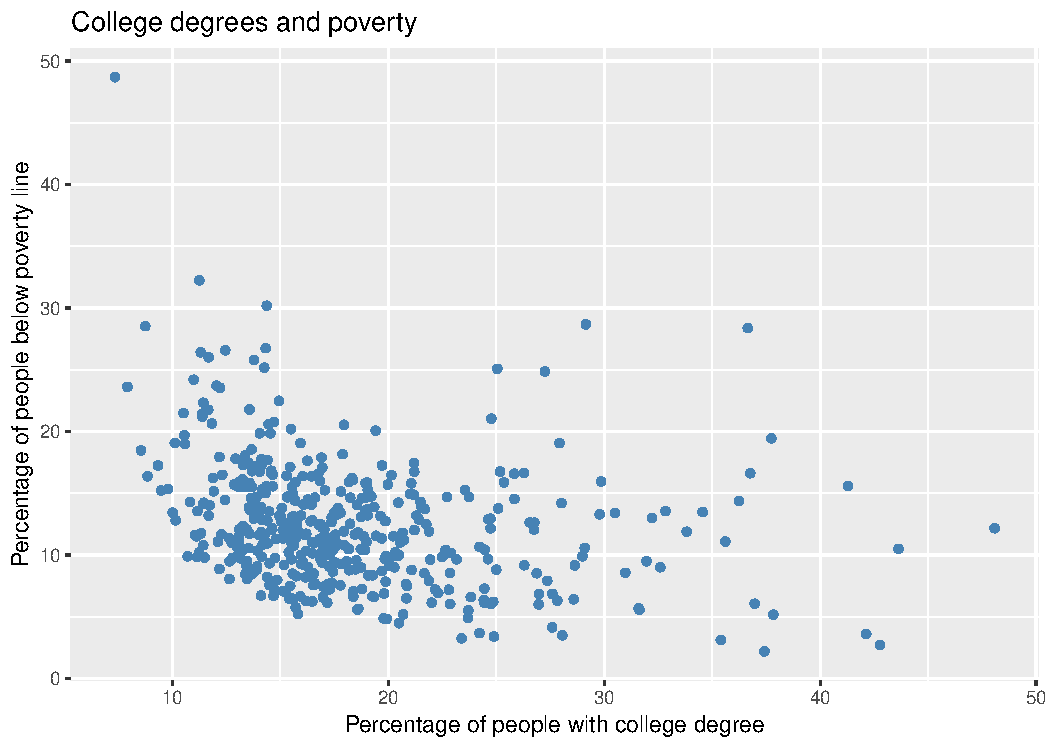
\includegraphics[width=4in]{plots/06.pdf} 
\end{figure}

Other things we can change are the background theme and the font size.

\begin{lstlisting}
> plot1 + 
+   theme_bw(20)
\end{lstlisting}

\begin{figure}[h]
\centering
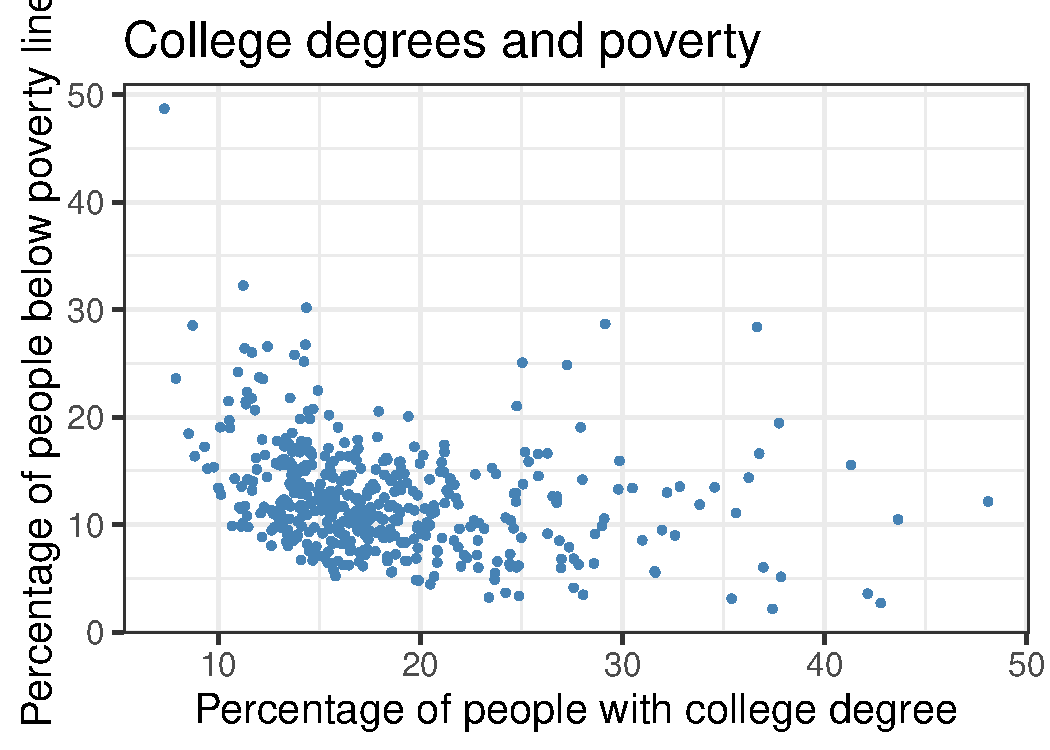
\includegraphics[width=4in]{plots/07.pdf} 
\end{figure}

\subsection{Adding features}

It is easy to add more features to a \texttt{ggplot}, just like we did with adding a title and axis labels. Now we'll add a best fit line, an arbitrary line, and a rug plot.

\begin{lstlisting}
> plot2 <- ggplot(midwest, aes(x = percollege, y = percbelowpoverty)) +
+            geom_point() +            
+            geom_smooth(method = "lm", size = 1) + # best fit line
+            geom_abline(intercept = 2, slope = 1
+                        , color = "red", size = 2) +
+            geom_rug(sides = "b")  # bottom rug plot
> plot2
\end{lstlisting}

\begin{figure}[h!]
\centering
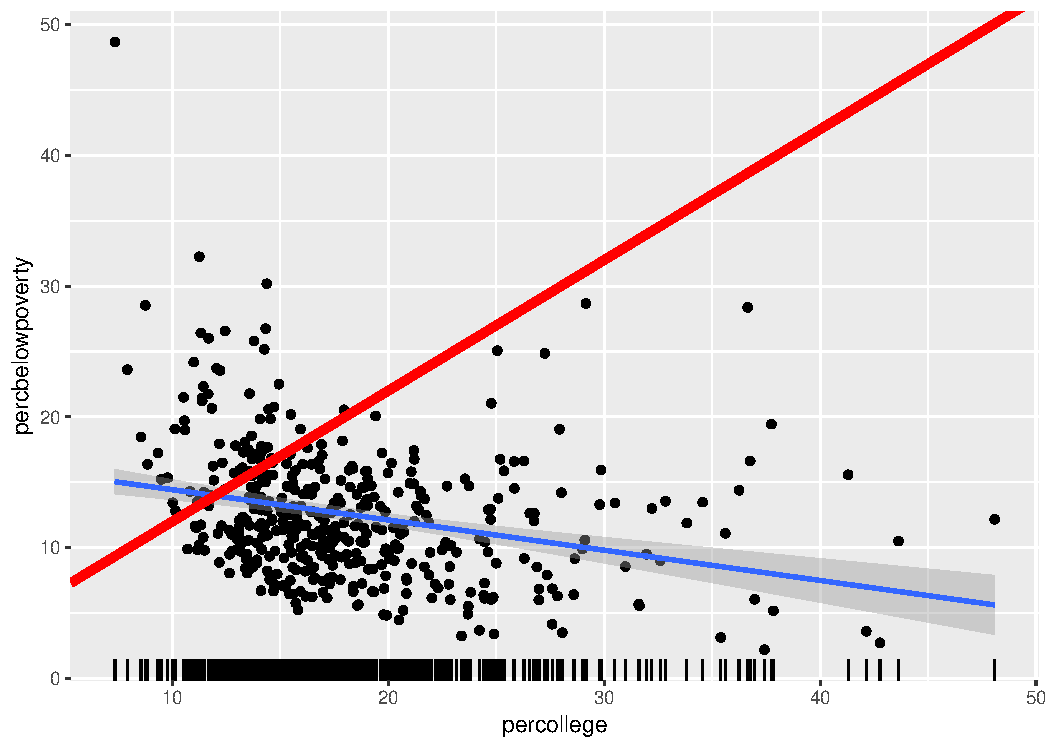
\includegraphics[width=4in]{plots/08.pdf} 
\end{figure}

\subsection{Other plots}

\subsubsection*{Histogram}

\begin{lstlisting}
> plot3 <- ggplot(midwest, aes(x = percollege)) +  # only need x for histogram
+             geom_histogram(binwidth = 1)
> plot3
\end{lstlisting}

\begin{figure}[h]
\centering
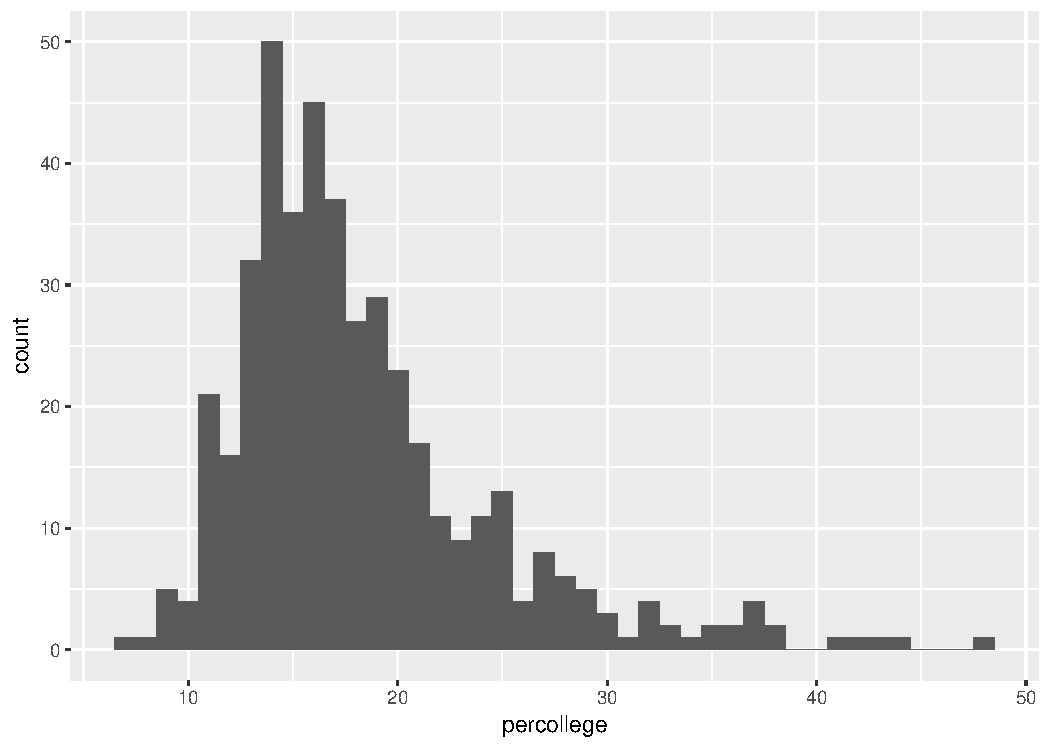
\includegraphics[width=4in]{plots/09.pdf} 
\end{figure}

I specified the bin width here, if you do not do that \R will choose something automatically. Let's change the colors and the axis labels.

\begin{lstlisting}
> plot3 <- plot3 +
+           geom_histogram(binwidth = 1
+                          , color = "black"  # outline
+                          , fill = "white")+ # inside
+           ylab("Count") +
+           xlab("Percentage of people with college degree")
> plot3
\end{lstlisting}

\begin{figure}[h]
\centering
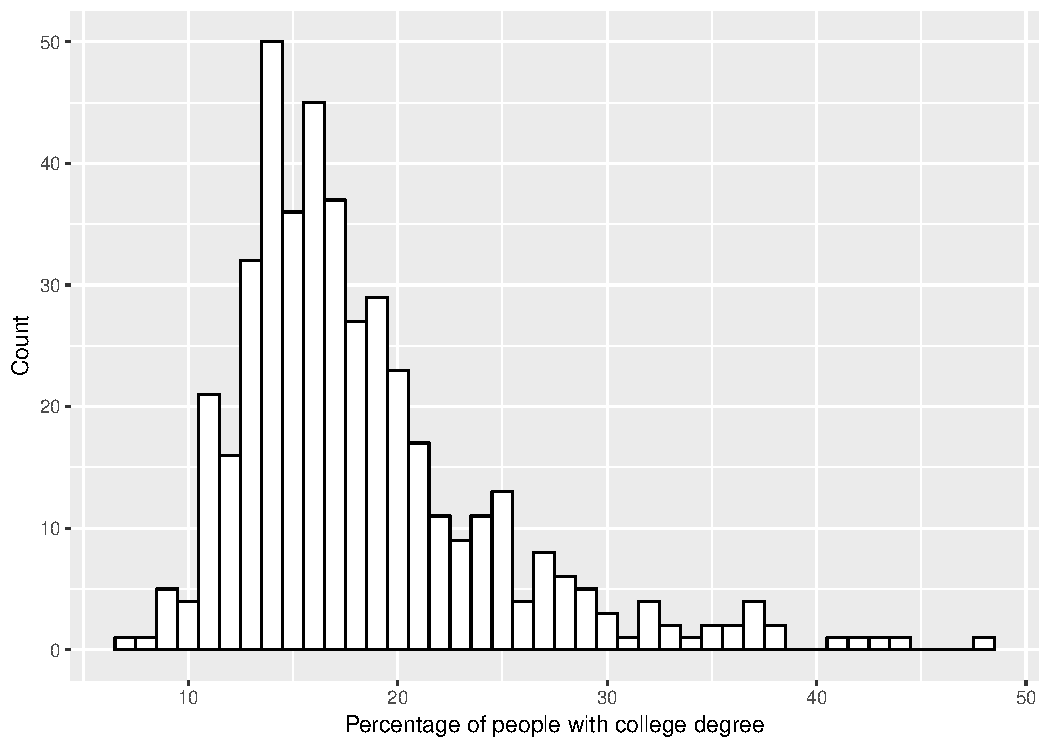
\includegraphics[width=4in]{plots/10.pdf} 
\end{figure}

\subsubsection*{Density}

A density plot is a smoothed version of the histogram for continuous data.

\begin{lstlisting}
> plot4 <- ggplot(midwest, aes(x = percollege)) + 
+             geom_density() +
+             ylab("Density") +
+             xlab("Percentage of people with college degree") +
+             ggtitle("Basic density")
> plot4
\end{lstlisting}

\begin{figure}[h]
\centering
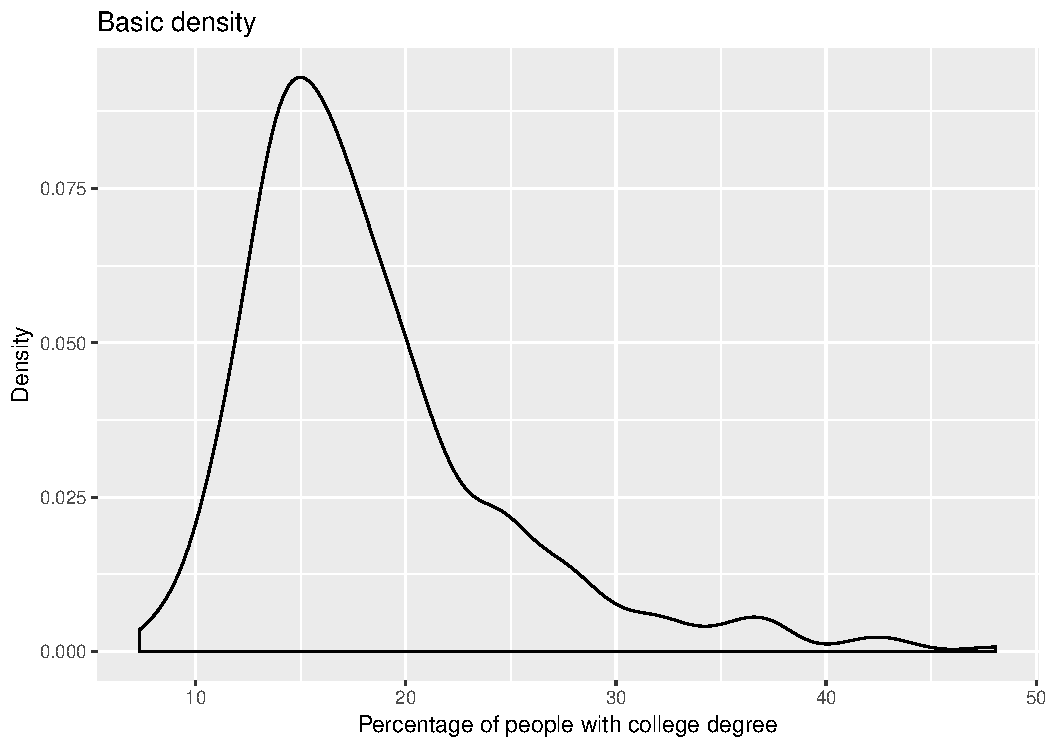
\includegraphics[width=4in]{plots/11.pdf} 
\end{figure}

We can check whether it matches the histogram by overlapping the two.

\begin{lstlisting}
> plot4 <-  ggplot(midwest, aes(x = percollege)) +
+           geom_histogram(aes(y =..density..)
+                          , binwidth = 1
+                          , color = "black"
+                          , fill = "white") +
+           geom_density(alpha = .2, fill = "#FF6666") +
+           ylab("Density") +
+           xlab("Percentage of people with college degree") +
+           ggtitle("Density + Histogram")
> plot4
\end{lstlisting}

\begin{figure}[h]
\centering
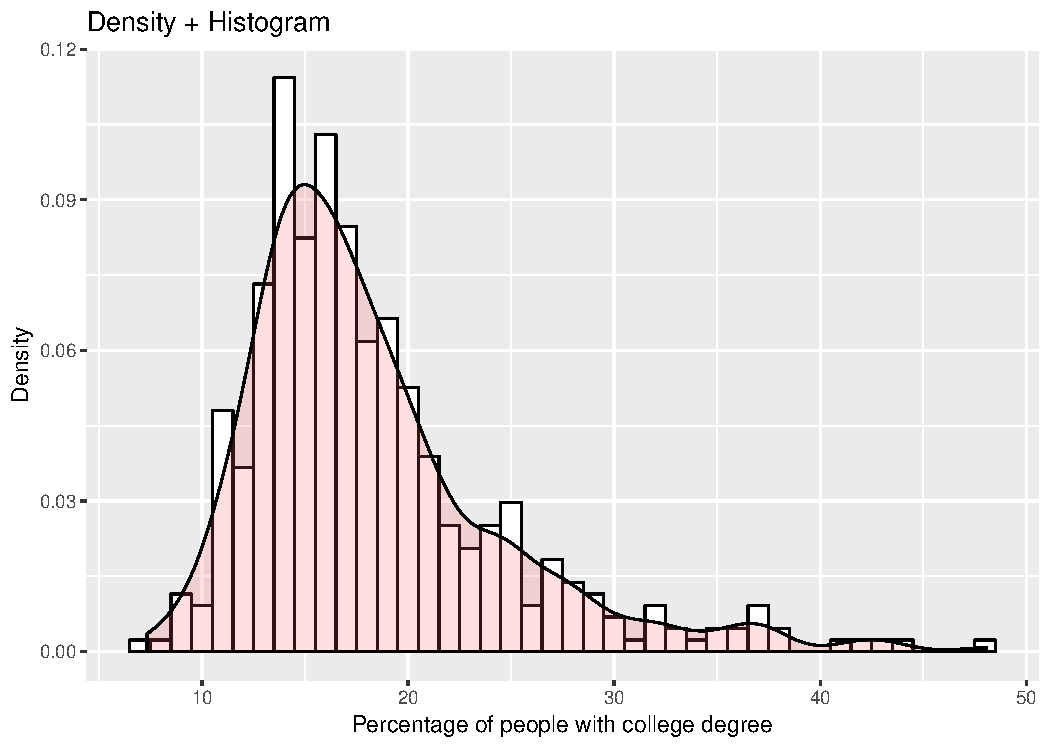
\includegraphics[width=4in]{plots/12.pdf} 
\end{figure}

\subsection{Saving plots}

To save individual plots you can do the following

\begin{lstlisting}
> ggsave(plot4, file = "plot4.pdf", height = 4, width = 6)  # saves into your working directory
\end{lstlisting}


